\begin{frame}\frametitle{Vehicle Navigation State Vector}
%The aim: accurate determination of the vehicle position and velocity
\begin{columns}
	\column{.62\textwidth}
	\textit{Vehicle state} is a vector that contains variables relevant for localising the vehicle (Eq. ~\ref{eq:state}). Vehicle navigation state describes its position and motion within the environment. Elements of the state vector $\vect{X}(k)$ are treated as Gaussian Random Variables (GRV). State vector will combine angular and metric values. \\
	{\footnotesize
	\begin{align}
		\vect{X}(k) = \left[ 
		\begin{array}{ccccccccccc}
		x & y & z & a & u & v & w & \psi & \varphi & \dot{\psi} & \dot{\varphi}
		\end{array} \right] ^{T}
		\label{eq:state}
	\end{align}
	}
{\footnotesize	
$\boldsymbol{x, y, z, a}$ : \textit{north}, \textit{east}, \textit{depth} and \textit{altitude} (Fig. \ref{fig:pos}). \\ 
$\boldsymbol{u, v, w}$ : linear velocities w.r.t sea bed in vehicle's coordinate system (\textit{surge}, \textit{sway} and \textit{heave}, Fig. \ref{fig:vel}) \\
$\boldsymbol{\psi, \varphi}$ : \textit{yaw} and \textit{pitch} (vehicle orientation, Fig. \ref{fig:pos}). \\
$\boldsymbol{\dot{\psi}, \dot{\varphi}}$ : \textit{yaw rate} and \textit{pitch rate} (angular velocities). 
} 
		
	\column{.35\textwidth}
	\begin{figure} %u, v, w - Velocity w.r.t sea bed in body coordinate
	\subfigure[velocities w.r.t. sea bed]{\label{fig:vel} 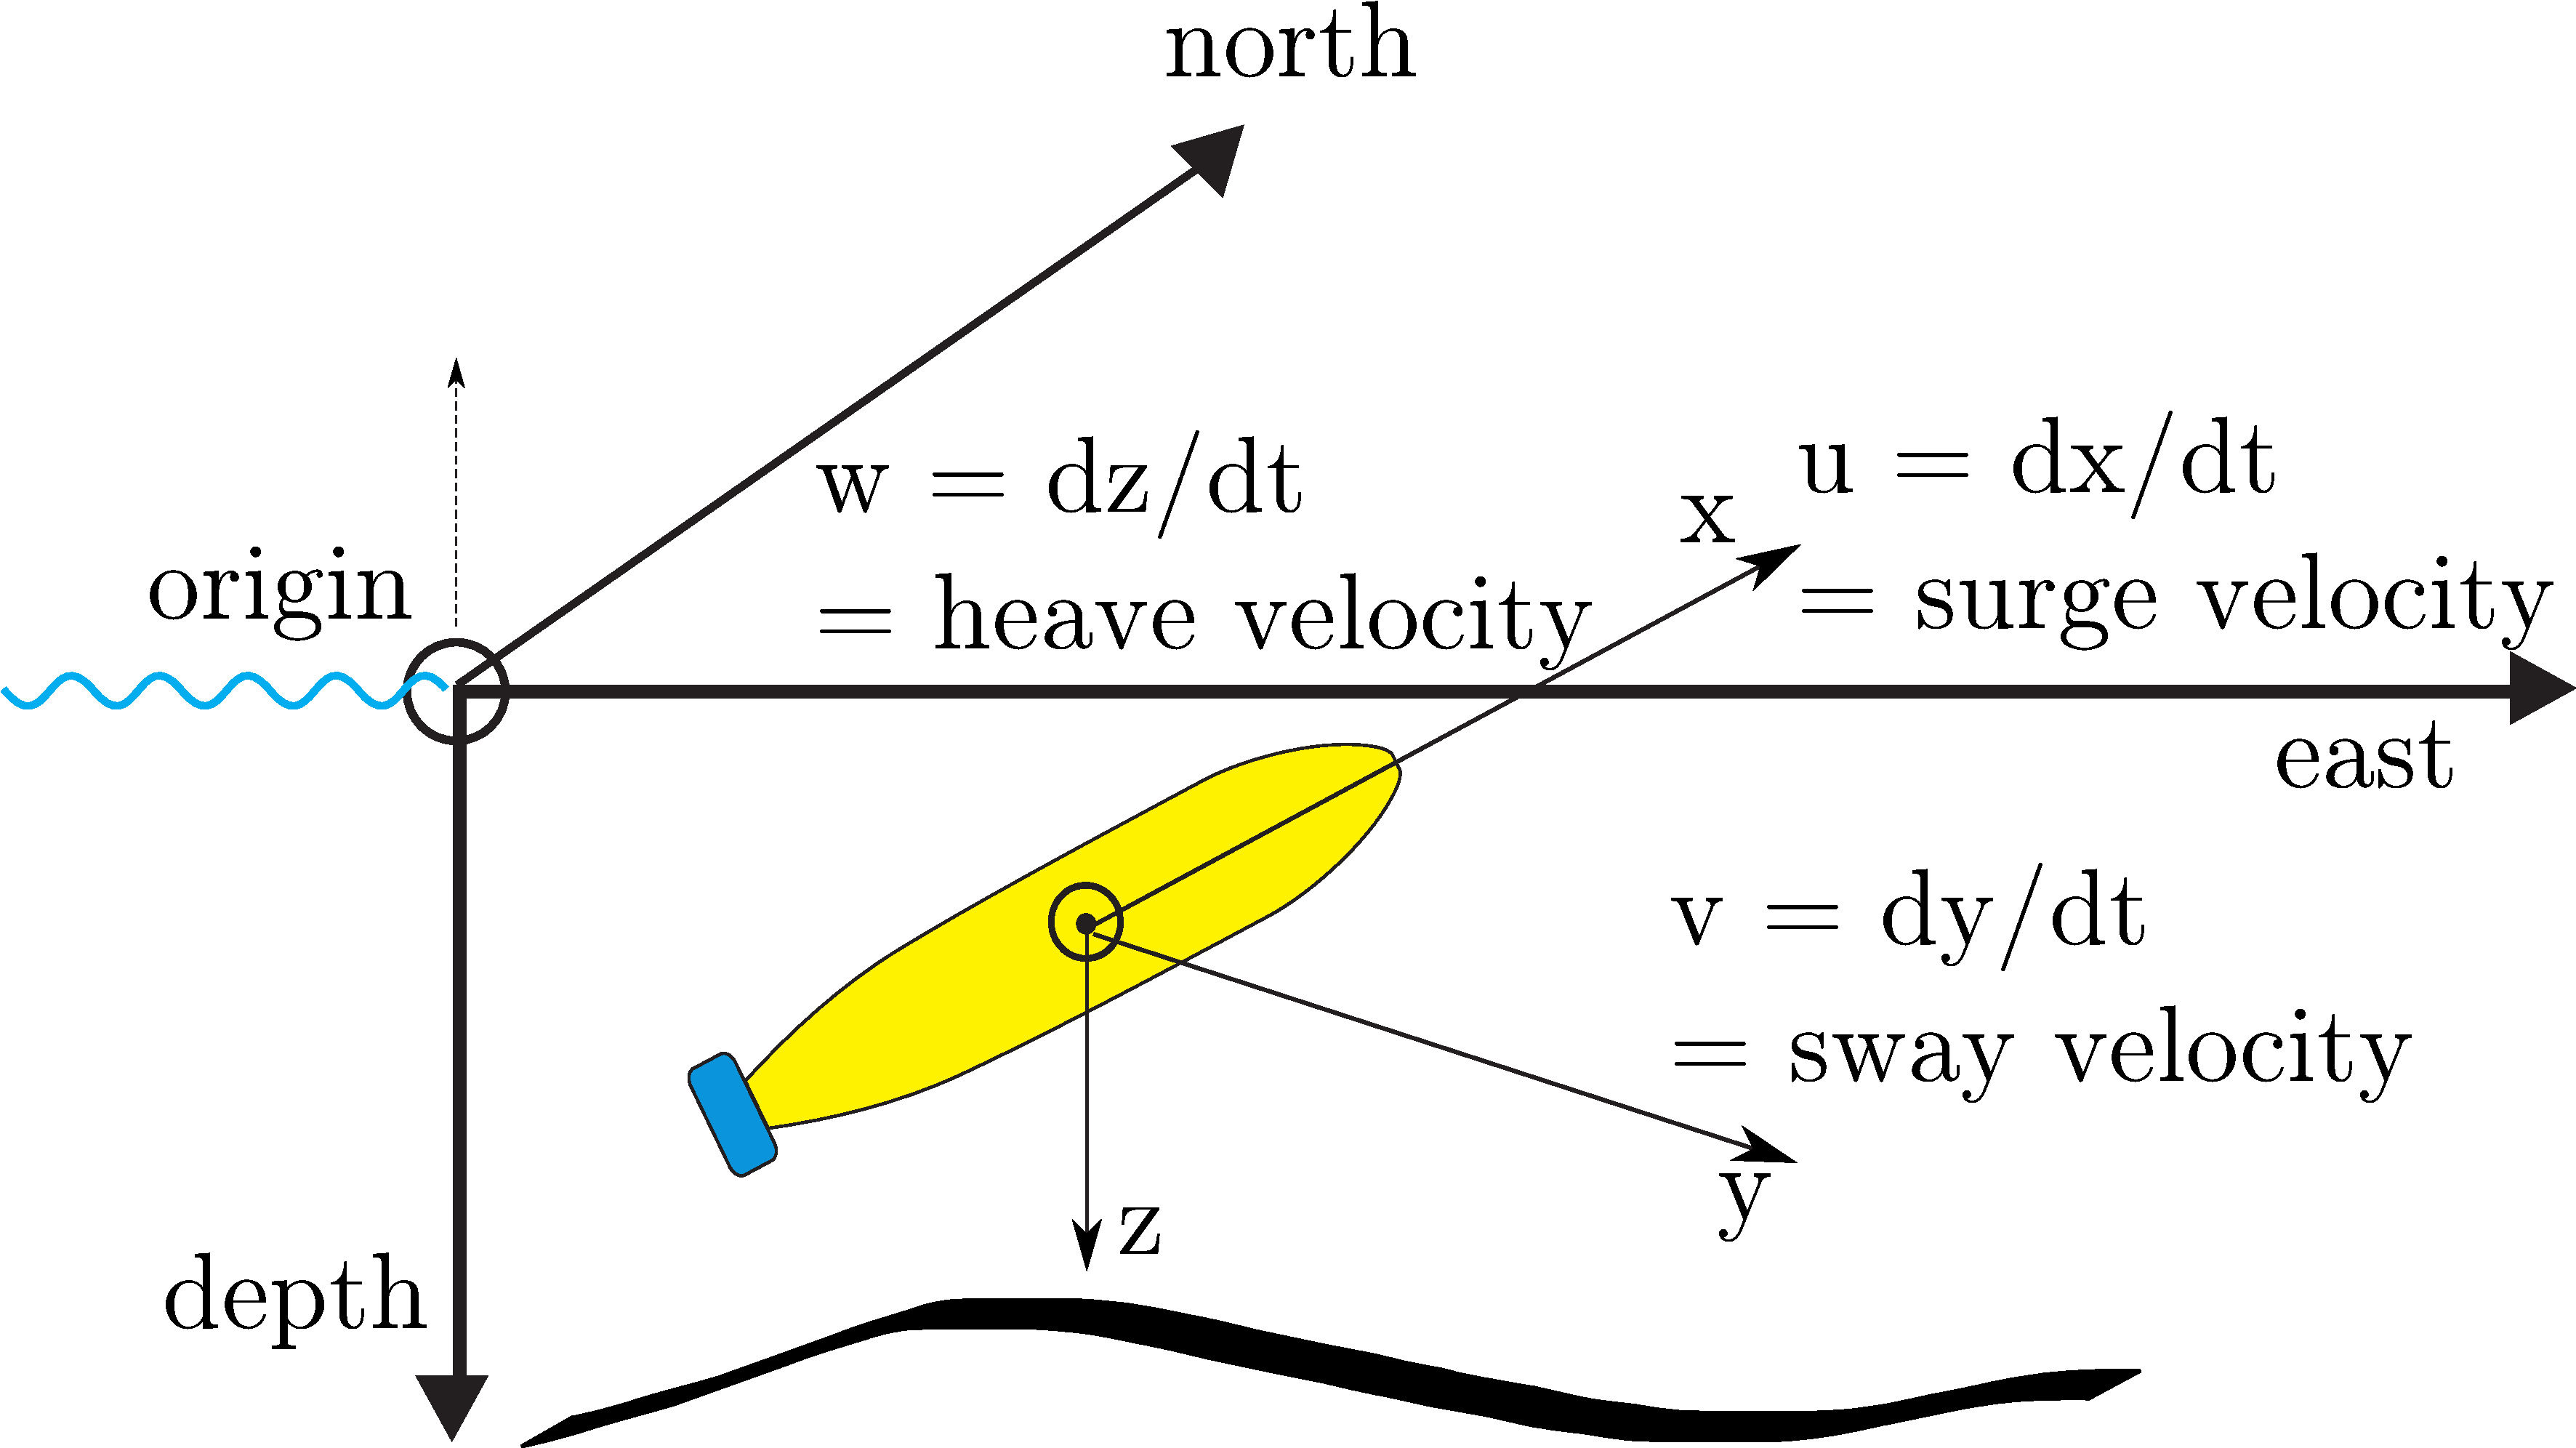
\includegraphics[width=0.95\linewidth]{fig/auv-axes.pdf}} \\
	\subfigure[global positioning]{\label{fig:pos} 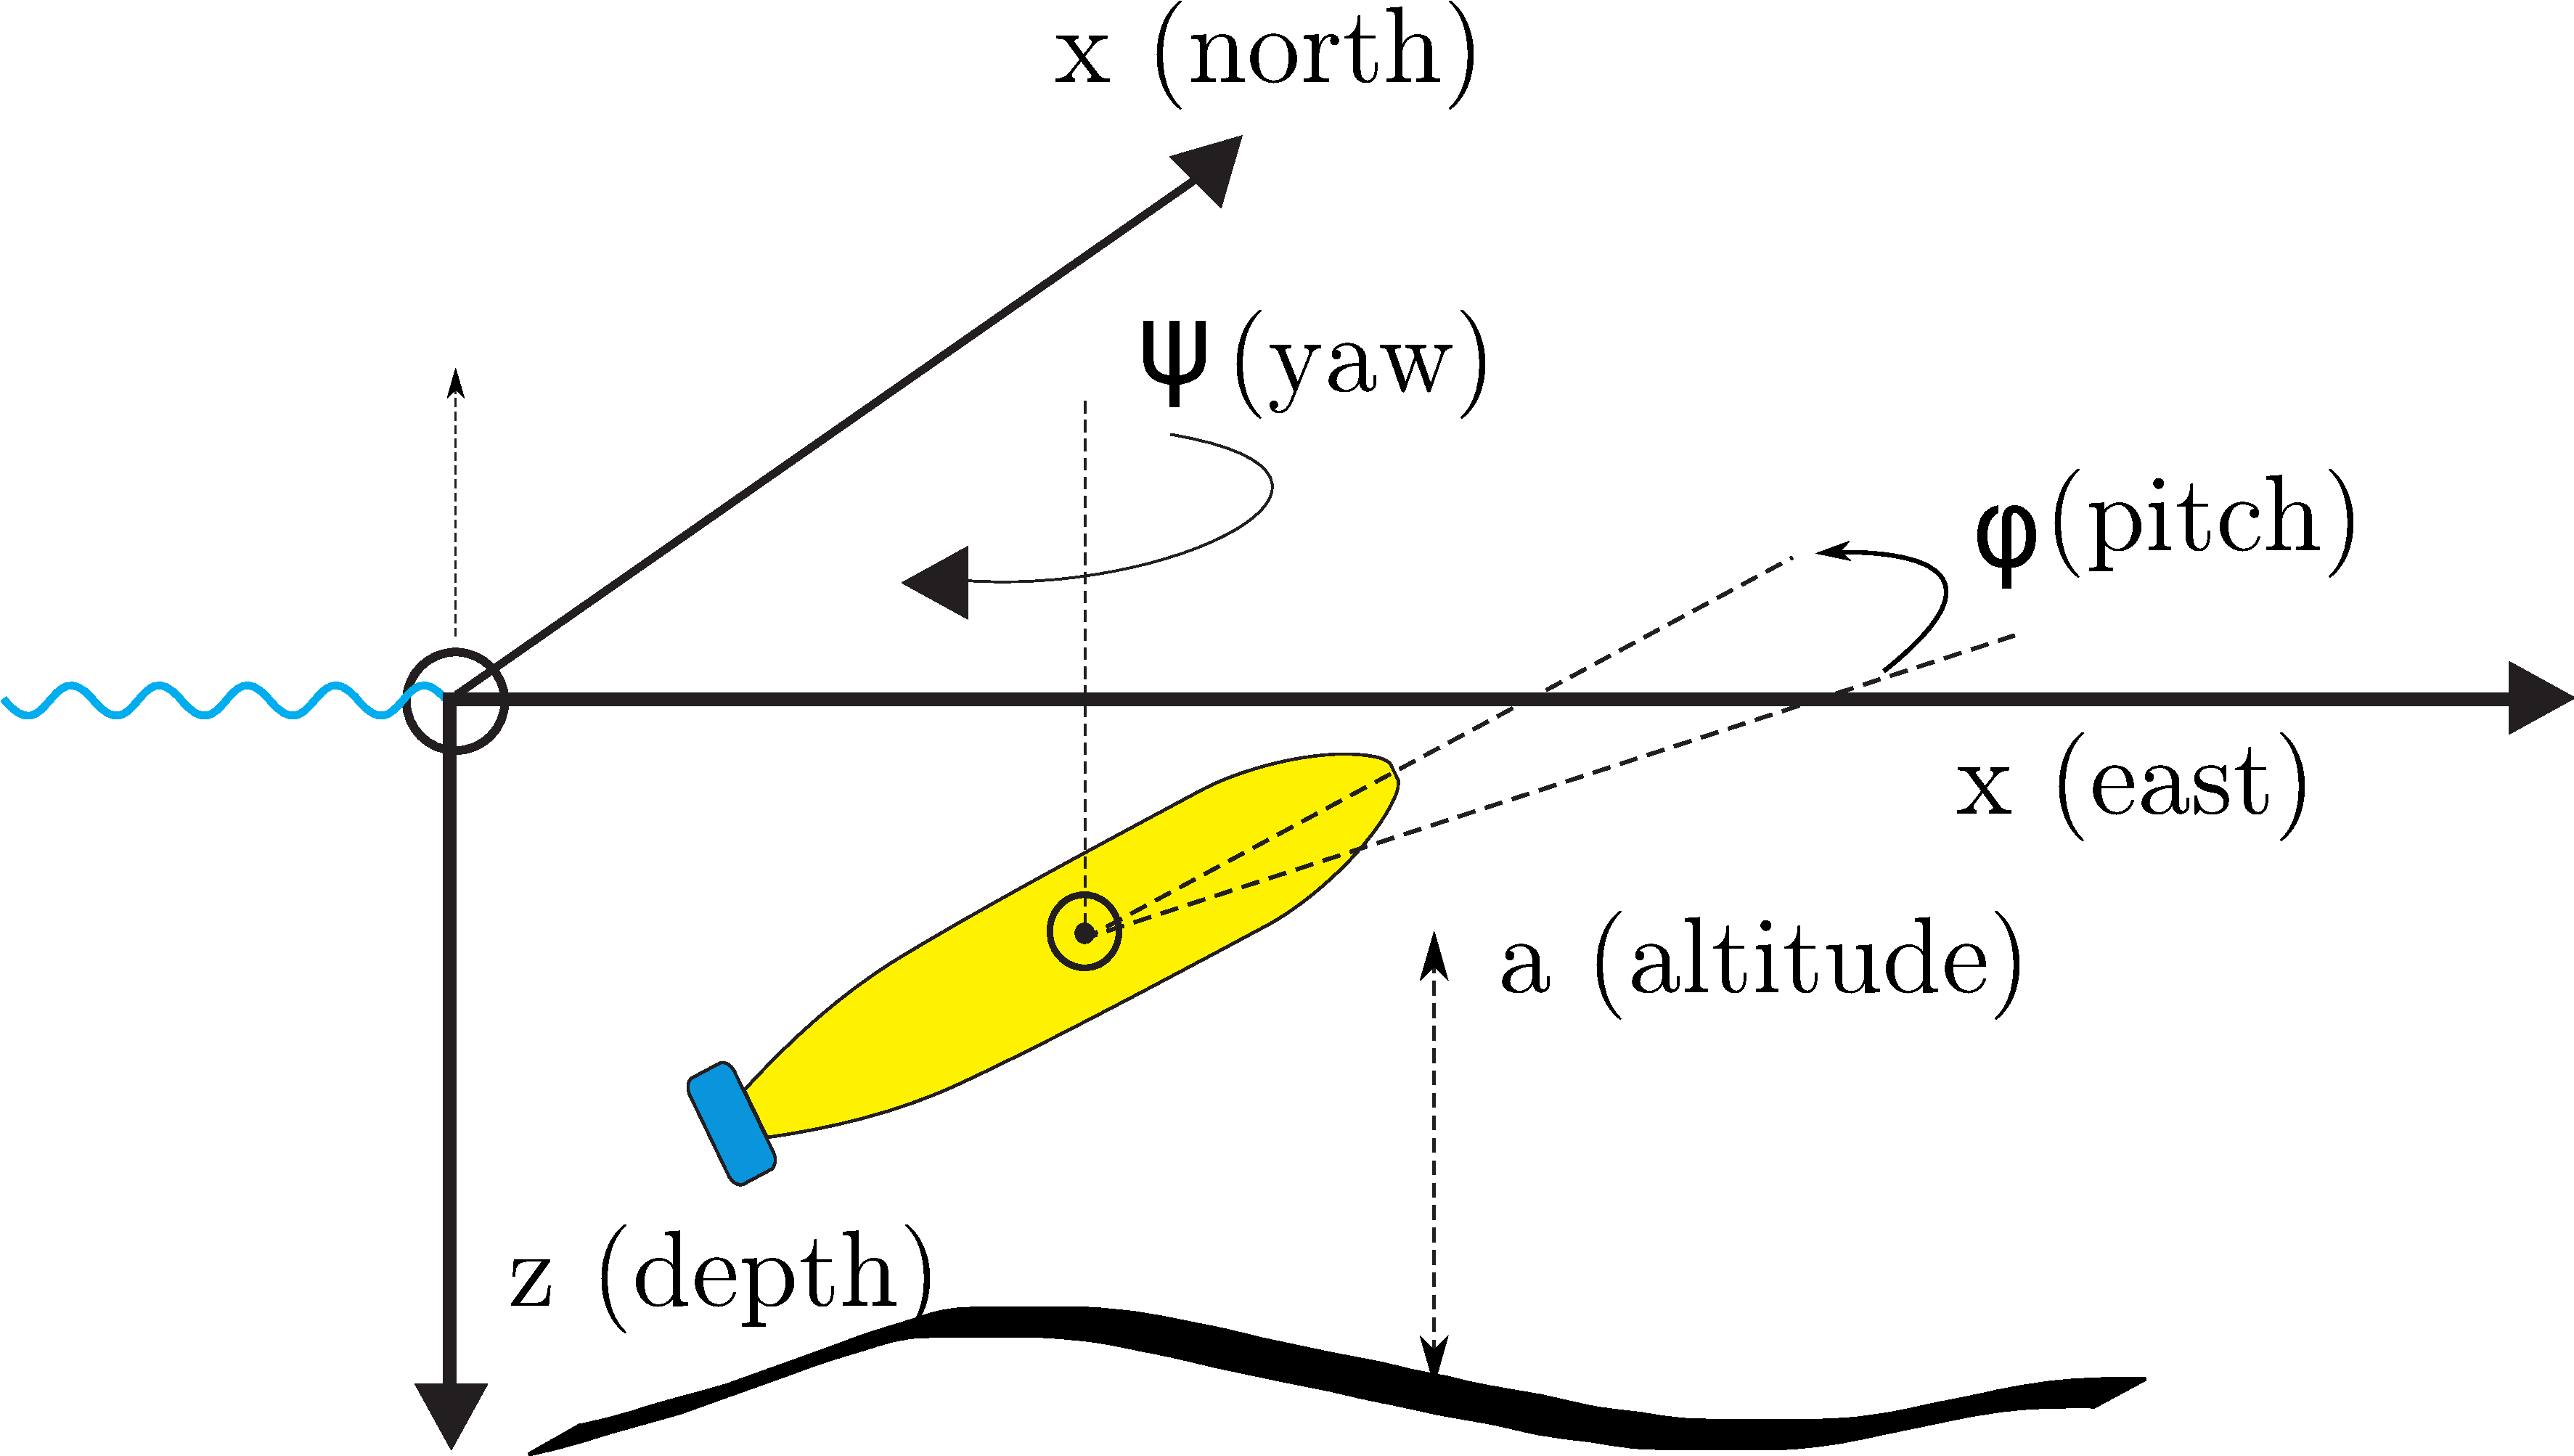
\includegraphics[width=0.95\linewidth]{fig/auv-model.pdf}}
	\caption{AUV positioning}
	\vspace{-25pt}
	\label{fig:positioning}
	\end{figure}
	
\end{columns}
\end{frame}

